% !TEX root = ../my-thesis.tex
%
\chapter{Data Analysis}
\label{sec:analysis}
In this chapter the models calculated for each country are reviewed. First, a look at the standardised incidence rate for each country is taken, before spatial models, spatio-temporal models and finally regression models are discussed.
\section{Standardised Incidence Ratio}
This section takes a brief look at the standardised incidence ratio for the countries of interest.
\subsection{Standardised Incidence Ratio for Germany}
When looking at the standardised incidence ratio for Germany, it is noticeable that the actual number of infections in the eastern parts of Germany, especially in Saxony, is considerably higher than the expected number of infections. Furthermore, parts of Bavaria have an increased standardised incidence ratio compared to the rest of Germany, excluding Saxony, see Figure~\ref{sirgermany}
% \begin{figure}[H]
%   \centering
%   \includesvg[width = 1.2\textwidth]{sir_germany.svg}
%   \caption{The standardised incidence ratio for Germany based on the data of the 5th of March 2021}
%   \label{sirgermany}
% \end{figure}
\begin{figure}[H]
  \centering
  \includegraphics[width = 1.2\textwidth]{sir_germany.png}
  \caption{The standardised incidence ratio for Germany based on the data of the 5th of March 2021}
  \label{sirgermany}
\end{figure}
\subsection{Standardised Incidence Ratio for Norway}
Looking at the standardised incidence rate for Norway, a standardised incidence rate of less than 1 can be seen for most municipalities north of Trondheim. In the southern parts of Norway there are several municipalities with a rate above 1, for example the standardised incidence rate around the capital Oslo is around 2. However, the two small municipalities, Hyllestad and Ulvik, have the highest standardised incidence rate in Norway. The SIR in Hyllestad is around 5, following an outbreak in a shipyard in autumn 2020 \cite{newspaper1}, while Ulvik has a ratio of around 9, following an outbreak of the UK variant of Covid-19. According to the head of the municipality, Hans Petter Thorbjørnsen, the infections are thought to have spread through children \cite{newspaper2}. See Figure~\ref{sirnorway} for more information.
% \begin{figure}[H]
%   \centering
%   \includesvg[width = 1.2\textwidth]{sir_norge.svg}
%   \caption{The standardised incidence ratio for Norway based on the data of the 5th of March 2021}
%   \label{sirnorway}
% \end{figure}
\begin{figure}[H]
  \centering
  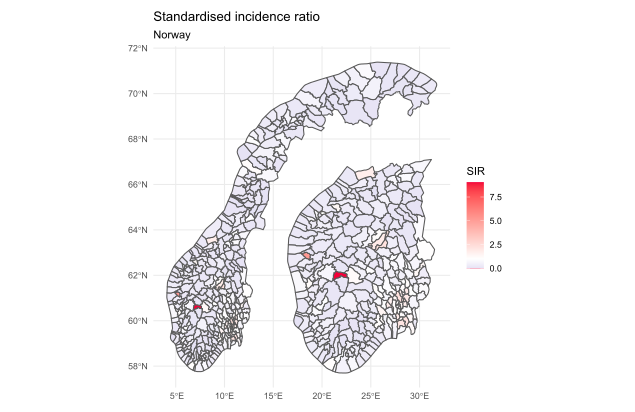
\includegraphics[width = 1.2\textwidth]{sir_norge.png}
  \caption{The standardised incidence ratio for Norway based on the data of the 5th of March 2021}
  \label{sirnorway}
\end{figure}
\clearpage
\section{Spatial Models}
After looking at the standardised incidence rates for the countries of interest, the next step is to take a closer look at the current figures for the respective countries. Spatial models are used to try to extract the factors that cause some populations to be at higher risk than other populations. Three different types of models are used for each country:
\begin{itemize}
    \item[1.] The Besarg-Yollie-Mollie Model
    \item[2.] Besags Proper Spatial Model
    \item[3.] The Leroux-Model
\end{itemize}
All of these models were computed using the INLA \cite{rinla} R package. \\
Before the models are computed, however, the distribution that fits the number of cases must first be found. For this, the function \texttt{descdist()} from the \texttt{fitdistrplus} R package is used. With this function, descriptive parameters of an empirical distribution can be calculated and a skewness-kurtosis plot is provided. The plots for Germany and Norway can be seen in Figure~\ref{cf_germany} and Figure~\ref{cf_norge}.
% \begin{figure}[H]
%     \centering
%     \includesvg[width = 0.8\textwidth]{cf-germany.svg}
%     \caption{The Cullen and Frey graph for Germany}
%     \label{cf_germany}
% \end{figure}
\begin{figure}[H]
    \centering
    \includegraphics[width = 0.8\textwidth]{cf-germany.png}
    \caption{The Cullen and Frey graph for Germany}
    \label{cf_germany}
\end{figure}
% \begin{figure}[H]
%     \centering
%     \includesvg[width = 0.8\textwidth]{cf_norge.svg}
%     \caption{The Cullen and Frey graph for Norway}
%     \label{cf_norge}
% \end{figure}
\begin{figure}[H]
    \centering
    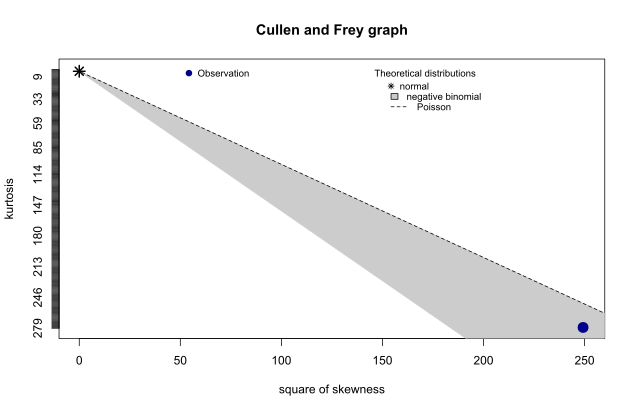
\includegraphics[width = 0.8\textwidth]{cf_norge.png}
    \caption{The Cullen and Frey graph for Norway}
    \label{cf_norge}
\end{figure}
Following these plots, a negative binomial distribution is fitted to the data using the maximum likelihood method. The function \texttt{fitdist()} is used for this. The fits can be seen in Figure~\ref{nb_germany} and Figure~\ref{nb_norge}.
% \begin{figure}[H]
%     \centering
%     \includesvg[width = 0.8\textwidth]{neg_binom_germany.svg}
%     \caption{A negative binomial fit to the number of cases in German municipalities}
%     \label{nb_germany}
% \end{figure}
\begin{figure}[H]
    \centering
    \includegraphics[width = 0.8\textwidth]{neg_binom_germany.png}
    \caption{A negative binomial fit to the number of cases in German municipalities}
    \label{nb_germany}
\end{figure}
% \begin{figure}[H]
%     \centering
%     \includesvg[width = 0.8\textwidth]{neg_binom_norge.svg}
%     \caption{A negative binomial fit to the number of cases in Norwegian municipalities}
%     \label{nb_norge}
% \end{figure}
\begin{figure}[H]
    \centering
    \includegraphics[width = 0.8\textwidth]{neg_binom_norge.png}
    \caption{A negative binomial fit to the number of cases in Norwegian municipalities}
    \label{nb_norge}
\end{figure}
Lastly, the AIC was calculated for fitting a normal distribution to the data, a Poisson distribution to the data and a negative binomial distribution to the data. The values can be seen in Table~\ref{aic}. Afterwards, the negative binomial distribution was chosen as the distribution of the target variable in both cases. \\
\begin{table}[H] 
\caption{THE AIC for different distributions for Germany and Norway \label{aic}}
\begin{tabular}{l l r}
\toprule
\textbf{Country}	& \textbf{Distribution}	& \textbf{AIC} \\
\midrule
Germany & Normal & 8364 \\
Germany & Poisson & 2065103 \\
Germany & Negative Binomial & 7726 \\
Norway & Normal & 6052 \\
Norway & Poisson & 314100 \\
Norway & Negative Binomial & 4018 \\
\bottomrule
\end{tabular}
\end{table} 
To specify each type of model, the following code shown in Listing~\ref{codeModels} can be used. \\
Three measures are used to compare the models, the DIC, the WAIC and the CPO. \\
For all countries, the models were computed with
\begin{itemize}
    \item[1.] only the demographic variables as covariates
    \item[2.] only the infrastructural variables as covariates
    \item[3.] both, demographic and infrastructural variables, as covariates
    \begin{itemize}
        \item[3.1] Without variable selection
        \item[3.2] With variable selection
    \end{itemize}
\end{itemize}
For each model type, different values for the penalised prior component were tried. As this resulted in a large number of models, only the model with the best performance for each model class is examined in more detail. To decide which models perform best, the DIC, WAIC and CPO are used. To select the best model, all calculated models were first ranked according to their DIC, their WAIC and their CPO before the model with the lowest average rank was selected as the best model. \\
Finally, due to the amount of covariates, forwards and backwards stepwise variable selection was performed with the intention of obtaining a model that fits the data well and at the same time is relatively easy to interpret. This can be done with the R package \texttt{INLAutils} \cite{inlautils}, as shown in Listing~\ref{codeSelection}. \\
A list of all calculated models along with their performance measures is provided in the appendix.
\subsection{Spatial Models for Germany}
First, a look is taken at the spatial models calculated for Germany. 
\subsubsection{Demographic Models}
The model with the best performance based on the demographic variables was a Leroux model calculated with the following formula:
\begin{lstlisting}[language=R]
formula_9_leroux <- CumNumberTestedIll ~
  trade_tax + income_total +
  f(
    idarea_1, model = "generic1",
    Cmatrix = C, hyper = prior_1
  )
\end{lstlisting}
The performance measures of this model and the best-performing BYM2 and Besag proper models are shown in Table~\ref{demoGermany}. A total of 66 models were calculated. The Leroux model had the best DIC and the fourth best CPO. Of all calculated models, the 20 best models in terms of the CPO were all Leroux models. The BYM2 model showed good performance in terms of the DIC and WAIC while Besags proper spatial model only showed good performance in terms of the WAIC.
\begin{table}[H] 
\caption{The performance measures for the best performing demographic model of each type. The rank in relation to each performance measure is shown in the brackets. \label{demoGermany}}
\begin{tabular}{l l l l}
\toprule
\textbf{Model}	& \textbf{DIC}	& \textbf{WAIC} & \textbf{CPO} \\
\midrule
Besags Proper  & 5696 (15) & 5603 (2) & -3358 (33) \\
BYM2 & 5639 (4) & 5578 (1) & -3375 (28)\\
Leroux & 5611 (1) & 5682 (18) & -3872 (2) \\
\bottomrule
\end{tabular}
\end{table}
The summary of the fixed effects is shown in Table~\ref{fixedDemoGermany}. To compute the posterior mean of the coefficients, the following code can be used:
\begin{lstlisting}[language=R]
inla.emarginal(exp, model_9_leroux$marginals.fixed$trade_tax)
# calculate the increase in risk if the 
# trade tax increase by 25000
inla.emarginal(
  exp,
  model_9_leroux$marginals.fixed$trade_tax
  ) ^ 25000
\end{lstlisting}
To obtain a credibility interval of the fixed effects on the original scale, the following code can be used:
\begin{lstlisting}[language=R]
inla.qmarginal(
  c(0.025,0.975),
  inla.tmarginal(
    exp,
    model_9_leroux$marginals.fixed$trade_tax
  )
)
\end{lstlisting}
\begin{table}[H] 
\caption{The fixed effects for model 10. Values are rounded. \label{fixedDemoGermany}}
\begin{tabular}{l r r r r}
\toprule
\textbf{Variable}	& \textbf{Mean}	& \textbf{exp(mean$_{\hbox{p}}$)} & \textbf{exp(q0025)} & \textbf{exp(q0975)} \\
\midrule
(Intercept) & 0.1483 & 1.1658 & 0.9604 & 1.4012\\
trade\_tax & 0.0000007026 & 1.000001  & 1.000000  & 1.000001 \\
income\_total & -0.00001633 & 0.9999837 & 0.9999729 & 0.9999944\\
\bottomrule
\end{tabular}
\end{table}
The posterior mean of the exponentiated intercept implies a 16.58\% risk rate across Germany with a credibility interval ranging from -3.96\% to 40.12\%.  \\
From this summary, it may seem difficult to interpret the impact of the trade tax and total income on the risk of contracting Covid-19, but it must be borne in mind that the difference in these variables is usually far greater than 1. \\
The range of the trade tax per 1000 inhabitants is from around 45000€ to 775000€. An increase in the trade tax by 25000€ per 1000 inhabitants leads to an increase in the risk of contracting Covid-19 by 1.77\%, given that the total income remains the same. \\
The range of total income, defined as the sum of income tax and payroll tax, per 1000 inhabitants ranges from 12500€ to about 36000€. An increase of 1000€ per 1000 inhabitants, with no change in trade tax, reduces the risk of contagion by about 1.62\%. \\
Since trade tax must be paid by all companies operating in Germany, this tax is highest in cities, as many companies have their headquarters there. This could therefore be an indication that the risk of infection is higher in cities. \\
On the other hand, the risk of infection decreases in regions where there is a higher total income based on payroll and income tax, i.e. where people earn a higher salary. Traditionally, people in western Germany have a higher income compared to eastern Germany, which could explain why eastern Germany, especially Saxony, is more affected by Covid-19 than some of the western parts of Germany.
\subsubsection{Infrastructure Models}
When it comes to the models based on the infrastructural variables, a BYM2 model performed the best. It was computed using the following formula: 
\begin{lstlisting}[language=R]
formula_26_bym2 <- CumNumberTestedIll ~
  marketplace + entertainment + sport + clinic +
  hairdresser + shops + place_of_worship + retail + nursing_home +
  restaurant + aerodrome + office + platform + schools + 
  higher_education + kindergarten + bakeries + 
  f(
    idarea_1, model = "bym2", graph = g,
    scale.model = TRUE, hyper = prior_2
  )
\end{lstlisting}
The performance measures of the computed models are shown in Table~\ref{infraGermany}. In total, 24 models were calculated.
\begin{table}[H] 
\caption{The performance measures for the best performing demographic model of each type. The rank in relation to each performance measure is shown in the brackets. \label{infraGermany}}
\begin{tabular}{l l l l}
\toprule
\textbf{Model}	& \textbf{DIC}	& \textbf{WAIC} & \textbf{CPO} \\
\midrule
Besags Proper & 5737 (12) & 5653 (3) & -3387 (13)\\
BYM2 & 5680 (1) & 5647 (2) & -3365 (20)\\
Leroux & 5699 (7) & 5681 (10) & -3568 (8) \\
\bottomrule
\end{tabular}
\end{table}
Again, the models with the best CPO were all Leroux models. \\
The effect of the covariates are shown in Table~\ref{fixedInfraGermany}.
\begin{table}[H] 
\caption{The fixed effects for the BYM2 model. Values are rounded. \label{fixedInfraGermany}}
\begin{tabular}{l r r r r}
\toprule
\textbf{Variable}	& \textbf{Mean}	& \textbf{exp(mean$_{\hbox{p}}$)} & \textbf{exp(q0025)} & \textbf{exp(q0975)} \\
\midrule
(Intercept) & 0.09038 & 1.100 & 0.9023 & 1.327\\
marketplace & 0.9468 & 3.293  & 0.6496  & 10.09 \\
entertainment & 0.3053 & 1.454 & 0.6566 & 2.798\\
hairdresser & 0.1362 & 1.154 & 0.9034 & 1.453\\
shops & 0.04251 & 1.058 & 0.7512 & 1.448\\
bakeries & 0.01805 & 1.031 & 0.7482 & 1.385\\
place\_of\_worship & -0.007848 & 0.9925 & 0.9445 & 1.042\\
platform & -0.01340 & 0.9867 & 0.9768 & 0.9966\\
nursing\_home & -0.02752 & 1.057 & 0.4365 & 2.160\\
schools & -0.02930 & 0.9764 & 0.7926 & 1.190\\
kindergarten & -0.03017 & 0.9772 & 0.7689 & 1.224\\
aerodrome & -0.03255 & 1.2162 & 0.2559 & 3.615\\
retail & -0.03583 & 0.9661 & 0.8700 & 1.070\\
restaurant & -0.04270 & 0.9587 & 0.8968 & 1.024\\
higher\_education & -0.07287 & 0.9363 & 0.7372 & 1.172\\
office & -0.08885  & 0.9172 & 0.7993 & 1.047\\
clinic & -0.09167 & 0.9135 & 0.8288 & 1.004\\
sport & -0.1211  & 0.8883 & 0.7693 & 1.020\\
\bottomrule
\end{tabular}
\end{table}
Some findings from these results are that the average risk ratio in Germany is 10\%. Marketplaces increase the risk by over 200\%, however, there is a maximum of only 0.1265 marketplaces per 1000 inhabitants, resulting in such a high value. If the number of marketplaces increases by 0.01 per 1000 inhabitants, the risk of infection increases by 1.20\%. More common sites that increase the risk of infection include bakeries (between 0.1169 and 0.9643 per 1000 inhabitants), hairdressers (between 0.09655 and 1.191 per 1000 inhabitants) and shops (between 0.3710 and 1.129 per 1000 inhabitants). An increase of 0.1 per 1000 for each of these types of establishments results in a risk increase of 0.3\%, 1.4\% and 0.6\%, respectively. It should not be surprising, in particular, that shops increase the risk of infection, as people tend to congregate there and people living in areas where a supermarket is nearby may prefer to go shopping more often in favour of fresh produce, rather than just once a week when a supermarket is further away. \\
There are also effects that have a posterior mean of less than 1, suggesting that they reduce the risk of infection. However, this is not necessarily the case, as it is probably safer for a person to stay at home rather than go to a restaurant, for example.
\subsubsection{Combined Models}
Finally, models are considered that include both the infrastructural and demographic covariates. Due to the amount of variables, all models run are based on variable selection. Since forwards and backwards variable selection was performed, a total of 12 models were run. The models with the best performance were a Leroux model that used forwards variable selection and a BYM2 model that used backwards variable selection. The difference between these types of variable selection can be seen in the Listing~\ref{formulaAllGermany}, as the Leroux model contains fewer variables.
\begin{lstlisting}[caption={The formulas for the best models containing all variables.}, label={formulaAllGermany}, language=R]
formula_31_bym2 <- CumNumberTestedIll ~
  asylum_seeker_benefits + trade_tax + 
  total_income + income_tax + Union + SPD + 
  FDP + die_linke + AfD + other_parties + protection_seekers +
  welfare_recipients +  unemployed_total + unemployed_foreigners +
  entertainment +  sport + clinic + hairdresser + shops +
  nursing_home + restaurant + aerodrome + platform + kindergarten +
  schools + bakeries +  pop_dens + urb_dens + sex +
  f(
    idarea_1, model = "bym2", graph = g,
    scale.model = TRUE, hyper = prior_1
  )
formula_34_leroux <- CumNumberTestedIll ~ 
  pop_dens + other_parties + SPD + 
  AfD + entertainment + unemployed_foreigners + unemployed_total + 
  welfare_recipients + schools + clinic +
  f(
    idarea_1, model = "generic1",
    Cmatrix = C, hyper = prior_2
  )
\end{lstlisting}
The performance measures of the computes models are shown in Table~\ref{allGermany}.
\begin{table}[H] 
\caption{The performance measures for the best performing demographic model of each type. The rank in relation to each performance measure is shown in the brackets. \label{allGermany}}
\begin{tabular}{l l l l}
\toprule
\textbf{Model}	& \textbf{DIC}	& \textbf{WAIC} & \textbf{CPO} \\
\midrule
Besags Proper & 6083 (9) & 6078 (9) & -3300 (11)\\
BYM2 & 5798 (3) & 5774 (3) & -3347 (5)\\
Leroux & 5815 (4) & 5827 (5) & -3551 (2) \\
\bottomrule
\end{tabular}
\end{table}
A look is only taken at the covariates of the Leroux model, as it has a lower CPO and is therefore better at predicting. The covariates of the BYM2 model are shown in Table~\ref{allGermanyBYM2} in the Appendix. For the Leroux model, the covariates are shown in Table~\ref{allGermanyLeroux}.

\begin{table}[H] 
\caption{The fixed effects for model 34. Values are rounded. \label{allGermanyLeroux}}
\begin{tabular}{l r r r r}
\toprule
\textbf{Variable}	& \textbf{Mean}	& \textbf{exp(mean$_{\hbox{p}}$)} & \textbf{exp(q0025)} & \textbf{exp(q0975)} \\
\midrule
(Intercept) & -0.244 & 0.7857 & -0.3993 & -0.08969\\
other\_parties & 29.01 & 1.176e+51  & -7.140  & 64.82 \\
AfD & 4.115 & 65.03 & 3.437 & 4.791\\
schools & 0.1743 & 1.198 & -0.05185 & 0.3999\\
unemployed\_ & \multirow{2}{*}{0.0611} & \multirow{2}{*}{1.063} & \multirow{2}{*}{0.04780} & \multirow{2}{*}{0.07443}\\
foreigners \\
pop\_dens & 0.00003913 & 1.000 & -0.00002088 & 0.00009896\\
clinic & -0.002106 & 0.9990 & -0.09274 & 0.08818\\
welfare\_ & \multirow{2}{*}{-0.01726} & \multirow{2}{*}{0.9829} & \multirow{2}{*}{-0.03298} & \multirow{2}{*}{-0.001590}\\
recipients \\
unemployed\_ & \multirow{2}{*}{-0.01744} & \multirow{2}{*}{0.9827} & \multirow{2}{*}{-0.02280} & \multirow{2}{*}{-0.01210}\\
total \\
entertainment & -0.6267 & 0.5732 & -1.361 & 0.1069\\
SPD & -1.666 & 0.1981  & -2.264 & -1.069\\
\bottomrule
\end{tabular}
\end{table}
What is immediately noticeable here is the extremely high coefficient for \textit{other\_parties}. However, one should bear in mind that in the 2019 European election the highest combined percentage of all other political parties was 0.4\%. Therefore, an increase of 0.005\% only increases the risk by 0.59\%. One of the larger political parties in Germany, the AfD, is known for its opposition to the corona rules in Germany. If the proportion of votes for this party increases by 1\% in a given area, the risk of getting Covid-19 increases by 4.26\%. Since the people who voted for them tend not to wear masks or keep a safe distance from others, it is not surprising that the infection figures are also higher in Bavaria and Saxony, both federal states where the AfD receives a higher proportion of the vote. The last positive effect worth mentioning is the number of schools per 1000 inhabitants. If these increase by 0.1, then the risk of infection increases by 1.8\%.
%%%%%%%%%%%%%% HIER GRAFIK
\subsection{Spatial Models for Norway}
Next, the same types of models are evaluated for Norway.
\subsubsection{Demographic Models}
As with Germany, the best demographic model was again a Leroux model. Only this time, the covariates of the model were selected using forwards variable selection. The following formula was used for the model:
\begin{lstlisting}[language = R]
formula_22_leroux <- value ~
  pop_dens + immigrants_pure + median_age +
  sex +
  f(
    idarea_1, model = "generic1",
    Cmatrix = C, hyper = prior_2
  )
\end{lstlisting}
The performance measures for all three types of models are shown in Table~\ref{demoNorway}.
\begin{table}[H] 
\caption{The performance measures for the best performing demographic model of each type. The rank in relation to each performance measure is shown in the brackets. \label{demoNorway}}
\begin{tabular}{l l l l}
\toprule
\textbf{Model}	& \textbf{DIC}	& \textbf{WAIC} & \textbf{CPO} \\
\midrule
Besags Proper  & 2804 (45) & 2820 (45) & -10433 (23) \\
BYM2 & 2716 (3) & 2670 (14) & -9786 (25)\\
Leroux & 2703 (1) & 2648 (1) & -11077 (14) \\
\bottomrule
\end{tabular}
\end{table}
The Leroux model had the best performance in terms of both DIC and WAIC and also performed well in terms of CPO. Just like for Germany, a total of 66 models were calculated. Of the 14 best models in terms of CPO, 13 were Leroux models. \\
The effects of the covariates are shown in Table~\ref{fixedDemoNorway}.
\begin{table}[H] 
\caption{The fixed effects for model 22. Values are rounded. \label{fixedDemoNorway}}
\begin{tabular}{l r r r r}
\toprule
\textbf{Variable}	& \textbf{Mean}	& \textbf{exp(mean$_{\hbox{p}}$)} & \textbf{exp(q0025)} & \textbf{exp(q0975)} \\
\midrule
(Intercept) & 1.087 & 222.4 & -4.681 & 6.826\\
pop\_dens & 0.001775 & 1.002 & 0.001048 & 0.002507\\
immigrants\_pure & -0.03358 & 0.9671 & -0.06291 & -0.005115\\
median\_age & -0.03628  & 0.9645 & -0.06242 & -0.01030\\
sex & -0.0426 & 2.902e+06 & -12.00 & 10.11 \\
\bottomrule
\end{tabular}
\end{table}
There is little meaningful interpretation for the posterior mean of the intercept in this model due to its high value. Of note is that if the population density increases by 10 persons per square kilometre, the risk of infection increases by about 1.8\%. Furthermore, if the proportion of women in an area increases by 0.05, the risk of infection increases by around 7.7\%. Finally, if the average age in a community increases by 1 year, the risk of infection decreases by roughly 3.5\%. Because younger people tend to be more mobile, they come into contact with more people than older generations, so it makes sense that people living in younger areas have a higher risk of becoming infected with Covid-19.
\subsubsection{Infrastructure Models}
\subsubsection{Combined Models}
\clearpage
\section{Spatio-Temporal Models}
\subsection{Spatio-Temporal Models for Germany}
\subsection{Spatio-Temporal Models for Norway}
\section{Regression Models}
\clearpage
\subsection{Regression Models for Germany}
\subsection{Regression Models for Norway}